\subsection{上同伦子的迷向群}

设 G 与 H 为群胚，\(\varphi\) 与 \(\psi\) 为从 H 到 G 的群胚态射。本节的目的，是计算上同伦子 \(\mathrm{Coh}(\varphi, \psi)\) 的迷向群。我们沿用第 3 号中的记号 \(G_1, h_1, \theta_1, \alpha, h\) 。

以 \(\Gamma_{0}\) 表示偶 \((\varphi,\psi)\) 的框架。回顾（II, 第 185 页, 定义 3），这是箭图 \((\mathrm{Orb}(\mathrm{G}),\mathrm{Orb}(\mathrm{H}),\varphi_{0},\psi_{0})\) ，其中 \(\varphi_{0}\) 与 \(\psi_{0}\) 是从 \(\mathrm{Orb}(\mathrm{H})\) 到 \(\mathrm{Orb}(\mathrm{G})\) 的、由映射 \(\varphi\) 与 \(\psi\) 通过取轨道诱导的映射。

在本节的余下部分，我们还将假设箭图 \(\Gamma_{0}\) 连通且非空；据 II, 第 185 页, 命题 4，这等价于假设群胚 \(\mathrm{Coh}(\varphi,\psi)\) 是传递的，或者等价地，箭图 \(G_{1}\) 连通且非空（II, 第 185 页, 命题 2）。

定义 4. —— 我们把下列数据称为偶 \((\varphi, \psi)\) 的基本配备：

\begin{enumerate}
\def\labelenumi{(\roman{enumi})}
\item
  对每个 \(i \in \mathrm{Orb}(\mathbf{G})\) ，取一个顶点 \(a(i)\) ，位于轨道 \(i\) （\(\mathbf{G}\) 的轨道）之中；
\item
  对每个 \(j \in \mathrm{Orb}(\mathrm{H})\) ，取一个顶点 \(b(j)\) ，位于轨道 \(j\) （H 的轨道）之中；
\item
  对每个 \(j \in \text{Orb(H)}\) ，取 G 中的箭 \(c_{1}(j)\) 与 \(c_{2}(j)\) ，分别连接 \(\varphi(b(j))\) 与 \(a(\varphi_{0}(j))\) 、\(\psi(b(j))\) 与 \(a(\psi_{0}(j))\) ；
\item
  框架 \(\Gamma_{0}\) 的一个子箭图 T，其相伴图是图 \(\widetilde{\Gamma}_{0}\) 的极大树；
\item
  G 的一个轨道 \(i_{0}\) 。
\end{enumerate}

选取一个基本配备 \((a,b,c_{1},c_{2},\mathrm{T},i_{0})\) （偶 \((\varphi,\psi)\) 的）。我们定义箭图态射 \(\tau_{1}\) （从 \(\Gamma_{0}\) 到 \(\operatorname{Grp}(\mathrm{G}_{1})\) ）如下：令 \(\tau_{1}(i)=a(i)\) （对 \(i\in\operatorname{Som}(\Gamma_{0})=\operatorname{Orb}(\mathrm{G})\) ），并令

\[
\tau_ {1} (j) = c _ {1} (j) ^ {- 1} \cdot h _ {1} (b (j)) \cdot c _ {2} (j)
\]

（对 \(j \in \mathrm{Fl}(\Gamma_{0}) = \mathrm{Orb}(\mathrm{H})\)）。以 \(\tau_{0}\) 表示 \(\tau_{1}\) 与典范态射 \(\theta_{1}\) （从 \(\mathrm{Grp}(\mathrm{G}_{1})\) 到 \(\mathrm{Coh}(\varphi, \psi)\) ）的复合；它是从 \(\Gamma_{0}\) 到 \(\mathrm{Coh}(\varphi, \psi)\) 的箭图态射。

对 \(i \in \mathrm{Orb}(\mathrm{G})\) ，以 \(\alpha_i \colon \mathrm{G}_{a(i)} \to \mathrm{Coh}(\varphi, \psi)_{a(i)}\) 表示由态射 \(\alpha \colon \mathrm{G} \to \mathrm{Coh}(\varphi, \psi)\) 通过限制到 \(a(i)\) 处的迷向群而得的群同态。

对 \(j\in \mathrm{Orb(H)}\) ，以

\[
\varphi_ {j} = \mathrm{Int} (c _ {1} (j)) ^ {- 1} \circ \varphi_ {b (j)} \colon \mathrm{H} _ {b (j)} \to \mathrm{G} _ {a (\varphi_ {0} (j))}
\]

及

\[
\psi_ {j} = \mathrm{Int} (c _ {2} (j)) ^ {- 1} \circ \psi_ {b (j)} \colon \mathrm{H} _ {b (j)} \to \mathrm{G} _ {a (\psi_ {0} (j))},
\]

表示相应的同态，使得对每个元素 \(f\) ∈ \(\mathrm{H}_{b(j)}\) ，有

\[
\varphi_ {j} (f) = c _ {1} (j) ^ {- 1} \varphi (f) c _ {1} (j) \quad \text { and } \quad \psi_ {j} (f) = c _ {2} (j) ^ {- 1} \psi (f) c _ {2} (j).\tag{6}
\]

对 \(\Gamma_{0}\) 的每个顶点 i，仍以 \(d_{i}\) 表示连接 \(i_{0}\) 与 i 的、树 \(\widetilde{T}\) 中的唯一道路类；把它看作 \(\mathrm{Grp}(\Gamma_{0})\) 中的一条箭。再以 \(\delta_{i}\) 表示 \(\mathrm{Coh}(\varphi,\psi)\) 中的这样一条箭：它是 \(d_{i}\) 在从 \(\mathrm{Grp}(\Gamma_{0})\) 到 \(\mathrm{Coh}(\varphi,\psi)\) 的、由 \(\tau_{0}\) 导出的典范态射下的像；\(\delta_{i}\) 的起点是 \(a(i_{0})\) ，其靶是 \(a(i)\) 。

箭图态射 \(\tau_0\) 、群同态 \(\alpha_i\) （对 \(i \in \mathrm{Orb}(\mathbf{G})\) ）、\(\varphi_j\) 与 \(\psi_j\) （对 \(j \in \mathrm{Orb}(\mathbf{H})\) ）、以及箭 \(\delta_i\) （在 \(\mathrm{Coh}(\varphi, \psi)\) 中）（对 \(i \in \mathrm{Orb}(\mathbf{G})\) ），称为由基本配备导出。

若 \((\mathrm{G}_{i})_{i\in\mathrm{I}}\) 是一族群，我们以 \(*G_{i}\) 表示它们的自由积；元素 \(g\in G_{i}\) 在从 \(G_{i}\) 到 \(*G_{i}\) 的典范映射下的像记作 {[}g{]} ，在无混淆可能时甚至记作 g。若 S 为集合，我们以 F(S) 表示在 S 上构造的自由群（A, I, 第 84 页）。

命题 6. —— 存在唯一的群同态

\[
\Lambda \colon \big (\underset {i \in \operatorname{Orb} (\mathrm{G})} {*} \mathrm{G} _ {a (i)} \big) * \mathrm{F} (\operatorname{Orb} (\mathrm{H})) \to \operatorname{Coh} (\varphi , \psi) _ {a (i _ {0})}
\]

使得

\begin{enumerate}
\def\labelenumi{(\arabic{enumi})}
\setcounter{enumi}{6}
\tightlist
\item
\end{enumerate}

\[
\Lambda (f) = \delta_ {i} \alpha_ {i} (f) \delta_ {i} ^ {- 1} \quad \text {   for   } i \in \operatorname{Orb} (\mathrm{G}) \text {   and   } f \in \mathrm{G} _ {a (i)},\tag{8}
\]

\[
\Lambda (j) = \delta_ {\varphi_ {0} (j)} \tau_ {0} (j) \delta_ {\psi_ {0} (j)} ^ {- 1} \qquad \text {for } j \in \mathrm{Orb} (\mathrm{H}).
\]

同态 \(\Lambda\) 是满射的；其核是 \((\ast_{i}\mathrm{G}_{a(i)})\ast\mathrm{F}(\mathrm{Orb}(\mathrm{H}))\) 的最小正规子群，它包含元素 \(j\) （属于 \(\mathrm{Fl}(\mathrm{T})\) ）以及诸元素 \(\varphi_{j}(f)j\psi_{j}(f)^{-1}j^{-1}\) （对 \(j\in\mathrm{Orb}(\mathrm{H})\) 及 \(f\in\mathrm{H}_{b(j)}\) ）。

同态 \(\Lambda\) 的存在性与唯一性由自由积与自由群的泛性质得出（A, I, 第 85 页, 命题 8）。

设 A 为诸 \(a(i)\) （对 \(i \in \mathrm{Orb}(\mathrm{G})\) ）的集合，并设 \(\mathrm{G}_{\mathrm{A}}\) 为 G 的以 A 为顶点集的全子群胚。对每个 \(x \in \text{Som(G)}\) ，以 \(\overline{x}\) 表示 \(x\) 在 G 中的轨道，并选取 G 的一条箭 \(d_x\) ，它连接 \(x\) 与 \(a(\overline{x})\) 。偶 \(v\) ——它由映射 \(x \mapsto a(\overline{x})\) （从 \(\text{Som(G)}\) 到 A 中的）以及把 \(f \in \text{Fl}_{x,y}(\text{G})\) 对应到元素 \(d_x^{-1}fd_y\) （属于 \(\text{Fl}_{a(\overline{x}),a(\overline{y})}(\text{G}_\text{A})\) ）的映射组成——是一个群胚态射。由 II, 第 182 页, 命题 1 推出，\(v\) 是同伦等价态射。令 \(\varphi' = v \circ \varphi\) 与 \(\psi' = v \circ \psi\) ，并以 \(w\) 表示从 \(\text{Coh}(\varphi, \psi)\) 到 \(\text{Coh}(\varphi', \psi')\) 的典范态射；它是同伦等价态射（II, 第 187 页, 定理 1）。

\(G_{A}\) 的轨道是诸集合 \(\{a\}\) （对 \(a \in A\) ），且单射 \(G_{A} \to G\) 诱导一个从 \(\mathrm{Orb}(G_{\mathrm{A}})\) 到 \(\mathrm{Orb}(G)\) 上的双射，我们将借此把这两个集合等同起来。定义基本配备 \((a', b', \beta_{1}', \beta_{2}', T', i_{0})\) （偶 \((\varphi', \psi')\) 的）如下：令 \(a'(i) = a(i)\) （对 \(i \in \mathrm{Orb}(G)\) ）、\(b'(j) = b(j)\) 、\(\beta_{1}'(j) = v(c_{1}(j))\) 、\(\beta_{2}'(j) = v(c_{2}(j))\) （对 \(j \in \mathrm{Orb}(H)\) ），并令 \(T' = T\) 。由这个基本配备导出的群同态 \(\varphi_{j}'\) 与 \(\psi_{j}'\) （对 \(j \in \mathrm{Orb}(H)\) ）、箭图态射 \(\tau_{0}'\) 、箭 \(\delta_{i}'\) （对 \(i \in \mathrm{Orb}(G)\) ）、从而还有群同态 \(\Lambda'\) ，分别是相应的同态 \(\varphi_{j}\) 、\(\psi_{j}\) 、箭图态射 \(\tau_{0}\) 、相应的箭 \(\delta_{i}\) 以及同态 \(\Lambda\) 与 w 的复合。

设 B 为诸 \(b(j)\) （对 \(j \in \mathrm{Orb}(\mathrm{H})\) ）的集合，并设 \(\mathrm{H}_{\mathrm{B}}\) 为 H 的以 B 为顶点集的全子群胚；以 \(u: \mathrm{H}_{\mathrm{B}} \to \mathrm{H}\) 表示典范单射；令 \(\varphi'' = \varphi' \circ u\) 与 \(\psi'' = \psi' \circ u\) 。态射 \(u\) 诱导一个双射 \(\mathrm{B} \to \mathrm{Orb}(\mathrm{H})\) ，我们将借此把这两个集合等同起来。我们再由 II, 第 187 页, 定理 1 得到一个典范同伦等价 \(w': \operatorname{Coh}(\varphi'', \psi'') \to \operatorname{Coh}(\varphi', \psi')\)。此外，偶 \((\varphi'', \psi'')\) 配备有一个基本配备 \((a'', b'', \beta_1'', \beta_2'', T'', i_0)\) ，使得 \(\Lambda', \varphi_j', \psi_j', \tau_0', \delta_i' (i, i' \in \operatorname{Orb}(\mathrm{G}), j \in \operatorname{Orb}(\mathrm{H}))\) 分别是 \(w'\) 与 \(\Lambda'', \varphi_j'', \psi_j'', \tau_0'', \delta_i'\) 的复合。

我们用下面的图表总结已引进的各个群胚态射：

\[
\begin{array}{c} \mathrm {H_ {B}} \xrightarrow [ \psi^ {\prime \prime} ]{\varphi^ {\prime \prime}} \mathrm {G_ {A}} \xrightarrow {\alpha^ {\prime \prime}} \mathrm{Coh} (\varphi^ {\prime \prime}, \psi^ {\prime \prime}) \\ \Big \downarrow \qquad \qquad \qquad \Big \| \qquad \qquad \qquad \Big \downarrow w ^ {\prime} \\ \mathrm{H} \xrightarrow [ \psi^ {\prime} ]{\varphi^ {\prime}} \mathrm {G_ {A}} \xrightarrow {\alpha^ {\prime}} \mathrm{Coh} (\varphi^ {\prime \prime}, \psi^ {\prime \prime}) \\ \Big \| \qquad \qquad \qquad \Big | _ {v} \qquad \qquad \qquad \Big | _ {w} \\ \mathrm{H} \xrightarrow [ \psi ]{\varphi} \mathrm{G} \xrightarrow {\alpha} \mathrm{Coh} (\varphi , \psi)  . \end{array}\tag{9}
\]

因此，为证明命题，我们可以假设 \(A = \text{Som}(G)\) 与 \(B = \text{Som}(H)\) ，换言之，典范映射 \(\text{Som}(G) \to \text{Orb}(G)\) 与 \(\text{Som}(H) \to \text{Orb}(H)\) 是双射；我们将在证明的余下部分在此假设之下进行。

这时箭图 \(G_{1}\) 以 A 为其顶点集，以诸集合 \(G_{a}\) （\(a \in A\)）与 B 的不交并为其箭集。\(G_{a}\) 的箭是 a 处的圈；若 \(b \in B\) ，则箭 b 连接 \(\varphi(b)\) 与 \(\psi(b)\) ，而箭 \(c_{1}(b)\) 与 \(c_{2}(b)\) 分别是 \(\varphi(b)\) 与 \(\psi(b)\) 处的圈。箭图 T 将与 \(G_{1}\) 的一个定向树等同起来；它是极大定向树，因为其顶点集等于 \(G_{1}\) 的顶点集（II, 第 157 页, 命题 1）。令 \(a_{0} = a(i_{0})\) 。框架 \(\Gamma_{0}\) （偶 \((\varphi, \psi)\) 的）的箭集既已等同于 B，箭图态射 \(\tau_{1}: \Gamma_{0} \to \text{Grp}(G_{1})\) 便把箭 b 对应到道路类 \(c_{1}(b)^{-1}bc_{2}(b)\) （在图 \(\widetilde{G_{1}}\) 中）。

回顾 \(\theta_{1}\) 表示从 \(\mathrm{G}_{1}\) 到 \(\mathrm{Grp}(\mathrm{G}_{1})\) 的典范箭图态射。以

\[
\lambda \colon \underset {a \in \mathrm{A}} {*} \mathrm{F} (\mathrm{G} _ {a}) * \mathrm{F} (\mathrm{B}) \to \operatorname{Grp} (\mathrm{G} _ {1}) _ {a _ {0}}
\]

表示唯一的群同态，使得

\[
\begin{array}{l l} \lambda (f) = \tau_ {1} (d _ {a}) \theta_ {1} (f) \tau_ {1} (d _ {a}) ^ {- 1} & \text {if } a\in A \text{ 且 } f\in G_{a} \text{;} \\ \lambda (b) = \tau_ {1} (d _ {\varphi (b)}) \tau_ {1} (b) \tau_ {1} (d _ {\psi (b)}) ^ {- 1} & \text {if } b\in B \text{.} \end{array}
\]

于是我们有 \(\lambda = \lambda' \circ \varepsilon\) ，其中 \(\lambda'\) 表示从 \(*_{a \in A} F(G_a) * F(B)\) 到 \(\text{Grp}(G_1)_{a_0}\) 的、由极大定向树 T 所定义的典范群同态（II, 第 179 页, 命题 9），而 \(\varepsilon\) 是群 \(*_{a \in A} F(G_a) * F(B)\) 的唯一自同构，满足 \(\varepsilon(f) = f\) （对 \(a \in A\) 及 \(f \in G_a\) ），以及 \(\varepsilon(b) = c_1(b)^{-1} h_1(b)c_2(b)\) （对 \(b \in B\) ）。由 II, 第 179 页, 注 2，同态 \(\lambda\) 是满射的，其核是 \(*_{a \in A} F(G_a) * F(B)\) 的包含 T 的诸箭的最小正规子群。

以 \(\pi\colon\mathrm{Grp}(\mathrm{G}_{1})\to\mathrm{Coh}(\varphi,\psi)\) 表示典范群胚态射。由 II, 第 177 页, 命题 8 的推论 1，群同态 \(\pi_{a_{0}}\) （从 \(\mathrm{Grp}(\mathrm{G}_{1})_{a_{0}}\) 到 \(\mathrm{Coh}(\varphi,\psi)_{a_{0}}\) ）是满射的，且其核是 \(\mathrm{Grp}(\mathrm{G}_{1})_{a_{0}}\) 的最小正规子群，它包含诸圈 \(\mathrm{Int}(\tau_{1}(d_{a}))( \alpha_{1}(f)\alpha_{1}(g)\alpha_{1}(fg)^{-1})\) （对 \(a\in\mathrm{A}\) 及 \(f,g\in\mathrm{G}_{a}\) ）以及诸圈 \(\mathrm{Int}(\tau_{1}(d_{\varphi(b)}))( \varphi(f)b\psi(f)^{-1}b^{-1})\) （对 \(b\in\mathrm{B}\) 及 \(f\in\mathrm{H}_{b}\) ）。

若以 \(p\colon F(\bigcup G_{a}\cup B)\to \left( \begin{array}{c} *\\ a\in A \end{array}G_{a}\right)*F(B)\) 表示典范满射同态，则我们有 \(\Lambda \circ p = \pi_{a_0}\circ \lambda\) 。这个公式蕴含同态 \(\Lambda\) 是满射的；剩下要确定它的核。

对 \(a \in \mathrm{A}\) 及 \(f \in \mathrm{G}_a\) ，以 {[}f{]} 表示 \(f \in \mathrm{F}(\mathrm{G}_a)\) 在群 \(*_{a \in \mathrm{A}} \mathrm{F}(\mathrm{G}_a) * \mathrm{F}(\mathrm{B})\) 中的像。那么，对 \(a \in \mathrm{A}\) 及 \(f, g \in \mathrm{G}_a\) ，我们有

\[
\operatorname{Int} \left(\tau_ {1} \left(d _ {a}\right)\right) \left(\alpha_ {1} (f) \alpha_ {1} (g) \alpha_ {1} (f g) ^ {- 1}\right) = \lambda ([ f ] [ g ] [ f g ] ^ {- 1}).
\]

类似地，对 \(b \in \mathrm{B}\) 及 \(f \in \mathrm{H}_b\) ，同态 \(\varphi_b\) 与 \(\psi_b\) 的定义（II, 第 193 页, 公式 (6)）蕴含

\[
\begin{array}{r l} & {\mathrm{Int} (\tau_ {1} (d _ {\varphi (b)})) (\varphi (f) h _ {1} (b) \psi (f) ^ {- 1} h _ {1} (b) ^ {- 1})} \\ & {\quad = \tau_ {1} (d _ {\varphi (b)}) \varphi (f) \big (c _ {1} (b) \tau_ {1} (b) c _ {2} (b) ^ {- 1} \big) \psi (f) ^ {- 1}} \\ & {\qquad \qquad \big (c _ {2} (b) \tau_ {1} (b) ^ {- 1} c _ {1} (b) ^ {- 1} \big) \tau_ {1} (d _ {\varphi (b)}) ^ {- 1}} \\ & {\quad = \tau_ {1} (d _ {\varphi (b)}) c _ {1} (b) \varphi_ {b} (f) \tau_ {1} (b) \psi_ {b} (f) ^ {- 1} \tau_ {1} (b) ^ {- 1} c _ {1} (b) ^ {- 1} \tau_ {1} (d _ {\varphi (b)}) ^ {- 1}} \\ & {\quad = \lambda (c _ {1} (b)) \lambda (\varphi_ {b} (f) [ b ] \psi_ {b} (f) ^ {- 1} [ b ] ^ {- 1}) \lambda (c _ {1} (b)) ^ {- 1}.} \end{array}
\]

因此，同态 \(\pi_{a_0} \circ \lambda\) 的核是 \(*\mathrm{F}(\mathrm{G}_a) * \mathrm{F}(\mathrm{B})\) 的最小正规子群，它包含元素 \([f][g][fg]^{-1}\) （对 \(a \in \mathrm{A}\) 及 \(f\) 、\(g \in \mathrm{G}_a\) ）、元素 \(\varphi_b(f)[b]\psi_b(f)^{-1}[b]^{-1}\) （对 \(b \in \mathrm{B}\) 及 \(f \in \mathrm{H}_b\) ）以及元素 \([b]\) （对 \(b \in \mathrm{Fl}(\mathrm{T})\) ）。

最后，同态 \(\Lambda\) 的核是 \((\underset{a\in\mathrm{A}}{*}\mathrm{G}_{a})*\mathrm{F}(\mathrm{B})\) 的最小正规子群，它包含前述诸元素在 \(p\) 下的像，换言之，即元素 \([b]\) （对 \(b\in\mathrm{Fl}(\mathrm{T})\) ）与元素 \(\varphi_{b}(f)[b]\psi_{b}(f)[b]^{-1}\) （对 \(b\in\mathrm{B}\) 及 \(f\in\mathrm{H}_{b}\) ）。命题得证。

\section{余均衡子}

\subsection{同伦箭的缩并}

设 H 为一个箭图，G 为一个群胚，\(\varphi\) 与 \(\psi\) 为从 H 到 G 的两个箭图态射，并设 \(h\colon \mathrm{Som}(\mathrm{H})\to \mathrm{Fl}(\mathrm{G})\) 为连接 \(\varphi\) 与 \(\psi\) 的一个同伦。设 G′ 为由 G 通过缩并 \(h\) 的像中的箭而得到的群胚（II, 第 175 页, 第 11 号），并设 \(\beta\colon\mathrm{G}\to\mathrm{G}'\) 为典范态射。

以 \(\Gamma\) 表示箭图 (Som(G), Som(H), Som(φ), Som(ψ))。根据同伦的定义，偶 (Id \(_{\text{Som(G)}}\) , \(h\) ) 是从 \(\Gamma\) 到 G 的一个箭图态射；它唯一地扩张为群胚态射 \(\eta\) : Grp(Γ) → G。根据构造，G′ 的顶点集是箭图 \(\Gamma\) 的连通分支所成的集。

在本节（\(n^{o}\)）的余下部分，我们将假设群胚 G 是传递的。由 II, 第 170 页的注 1，这等价于假设群胚 G′ 是传递的。我们还固定 G 的一个顶点 \(a_{0}\) 。

以 \(\widetilde{\Gamma}\) 表示与箭图 \(\Gamma\) 相伴的图（参看 II, 第 156 页）。长度 \(\geqslant 1\) 的回路（\(\widetilde{\Gamma}\) 中的）所成的集与集 \(\Omega(\widetilde{\Gamma})\) （有限序列 \((z_1, \ldots, z_n)\) 所成之集）等同，其中 \(n\) 是满足 \(n \geqslant 1\) 的整数，而 \(z_1, \ldots, z_n\) 是 \(\mathrm{Fl}(\widetilde{\Gamma})\) 的元素，满足 \(t(z_i) = o(z_{i+1})\) （对每个整数 \(i\) ，满足 \(1 \leqslant i < n\) ）以及 \(t(z_n) = o(z_1)\) 。

设 \(\mathbf{z} = ((b_{1}, \varepsilon_{1}), \ldots, (b_{n}, \varepsilon_{n}))\) 为 \(\Omega(\widetilde{\Gamma})\) 的一个元素。元素

\[
\operatorname{Int} (g) (\eta (\mathbf {z})) = g h (b _ {1}) ^ {\varepsilon_ {1}} \dots h (b _ {n}) ^ {\varepsilon_ {n}} g ^ {- 1}
\]

在 \(G_{a_{0}}\) 中的共轭类不依赖于 G 的、连接顶点 \(a_{0}\) 与 \((b_{1},\varepsilon)\) 的起点的箭 g 的选取。我们以 \(c(\mathbf{z})\) 表示此共轭类。

命题 1. —— 群同态 \(\beta_{a_0} \colon \mathrm{G}_{a_0} \to \mathrm{G}'_{\beta(a_0)}\) 是满射的，其核是 \(\mathrm{G}_{a_0}\) 的、包含共轭类 \(c(\mathbf{z})\) （对 \(\mathbf{z} \in \Omega(\widetilde{\Gamma})\) ）的最小子群。

设 K 为 G 的最小的正规子群胚，其箭集包含 h 的像。态射 \(\mathrm{G}_{a_{0}} \rightarrow \mathrm{G}^{\prime}_{\beta(a_{0})}\) 是满射的，且其核等于 \(K_{a_{0}}\) （II, 第 170 页, 命题 2）。于是命题由 II, 第 176 页的命题 8 得出。

定义 1. —— 称 \(\Omega(\widetilde{\Gamma})\) 的一个子集 Z 为正规的（相对于偶 \((\varphi, \psi)\) ），如果它满足下列性质：

\begin{enumerate}
\def\labelenumi{(\roman{enumi})}
\item
  对 Γ 的每条箭 z，有 \((z,\overline{z})\in\mathbb{Z}\) ；
\item
  对每个 \((z_{1},\ldots ,z_{n})\in \mathbb{Z}\) ，我们有 \((\overline{z}_n,\dots ,\overline{z}_2,\overline{z}_1)\in \mathbb{Z}\) 以及 \((z_{n},z_{1},\ldots ,z_{n - 1})\in \mathbb{Z}\) ；
\item
  设 \(\mathbf{z} = (z_1, \ldots, z_n)\) 与 \(\mathbf{z}' = (z_1', \ldots, z_m')\) 为 \(Z\) 中满足 \(t(z_n) = o(z_1')\) 的元素。令 \(\mathbf{z}\mathbf{z}' = (z_1, \ldots, z_n, z_1', \ldots, z_m')\) 。若 z、z′、zz′ 三者中有两个属于 Z，则第三个也属于 Z；
\item
  对 H 的每条箭 \(f\) ，令 \(\widetilde{\varphi}(f,1) = \widetilde{\psi}(f,-1) = \varphi(f)\) 以及 \(\widetilde{\varphi}(f,-1) = \widetilde{\psi}(f,1) = \psi(f)\) 。设 \(n\) 为一个整数 \(\geqslant 1\) ，并设 \((f_1,\varepsilon_1),\ldots,(f_n,\varepsilon_n)\) 为 \(\mathrm{Fl}(\mathrm{H})\times \{-1,1\}\) 的元素的一个序列，满足 \(\widetilde{\psi}(f_i,\varepsilon_i) = \widetilde{\varphi}(f_{i+1},\varepsilon_{i+1})\) （对 \(1\leqslant i < n\) ）以及 \(\widetilde{\psi}(f_n,\varepsilon_n) = \widetilde{\varphi}(f_1,\varepsilon_1)\) ；以 \(a_i\) 表示 \(f_i\) 的起点，以 \(b_i\) 表示其靶。\(((a_1,\varepsilon_1),\ldots,(a_n,\varepsilon_n))\) 属于 Z 当且仅当 \(((b_1,\varepsilon_1),\ldots,(b_n,\varepsilon_n))\) 属于 Z。
\end{enumerate}

\(\Omega(\widetilde{\Gamma})\) 中任意一族正规子集（相对于 \((\varphi, \psi)\) ）的交仍是正规的。特别地，对给定子集 \(Z\) （\(\Omega(\widetilde{\Gamma})\) 的），存在包含它的最小正规子集。

命题 2. —— 若 \(N\) 是 \(G_{a}\) 的一个正规子群，则元素 \(\mathbf{z} \in \Omega(\widetilde{\Gamma})\) （满足 \(c(\mathbf{z})\) 包含于 \(N\) ）所成的集是 \(\Omega(\widetilde{\Gamma})\) 的一个正规子集。

以 Z 表示元素 \(\mathbf{z} \in \Omega(\widetilde{\Gamma})\) （满足 \(c(\mathbf{z}) \subset \mathrm{N}\) ）所成的集。

设 \(z \in \mathrm{Fl}(\widetilde{\Gamma})\) 。根据定义有 \(c(z, \overline{z}) = \{e_a\}\) ，从而 \((z, \overline{z}) \in \mathbf{Z}\) 。设 \((z_1, \ldots, z_n) \in \mathbf{Z}\) 。根据 \(c\) 的定义，共轭类 \(c(z_1, \ldots, z_n)\) 等于 \(c(z_n, z_1, \ldots, z_{n-1})\) ，并且由 \(c(\overline{z}_n, \ldots, \overline{z}_1)\) 的元素的逆所组成。这表明 \(\mathbf{Z}\) 满足条件 (ii)。

采用条件 (iii) 的记号，可以选取元素 \(u \in c(\mathbf{z})\) 、\(v \in c(\mathbf{z}')\) 与 \(w \in c(\mathbf{z}\mathbf{z}')\) ，使得 uv = w。若元素 u、v 与 w 三者中有两个属于 N，则第三个亦然，因此 N 满足 (iii)。

采用 (iv) 中的记号，对每个满足 \(1 \leqslant i \leqslant n\) 的整数 i，有关系式

\[
  \varphi (f _ {i}) h (b _ {i}) = h (a _ {i}) \psi (f _ {i}),
\]

因为 h 是连接 \(\varphi\) 与 \(\psi\) 的一个同伦。此等式也可写成

\[
\widetilde {\varphi} (f _ {i}, \varepsilon_ {i}) h (b _ {i}) ^ {\varepsilon_ {i}} = h (a _ {i}) ^ {\varepsilon_ {i}} \widetilde {\psi} (f _ {i}, \varepsilon_ {i}).
\]

考虑到关系式 \(\widetilde{\psi}(f_i,\varepsilon_i) = \widetilde{\varphi}(f_{i + 1},\varepsilon_{i + 1})\) （对 \(1\leqslant i <   n\) ）以及 \(\widetilde{\psi} (f_n,\varepsilon_n) = \widetilde{\varphi} (f_1,\varepsilon_1)\) ，我们推出

\[
\widetilde {\varphi} (f _ {1}, \varepsilon_ {1}) h (b _ {1}) ^ {\varepsilon_ {1}} \dots h (b _ {n}) ^ {\varepsilon_ {n}} = h (a _ {1}) ^ {\varepsilon_ {1}} \dots h (a _ {n}) ^ {\varepsilon_ {n}} \widetilde {\varphi} (f _ {1}, \varepsilon_ {1}),
\]

从而共轭类 \(c((a_{1},\varepsilon_{1}),\ldots,(a_{n},\varepsilon_{n}))\) 与 \(c((b_{1},\varepsilon_{1}),\ldots,(b_{n},\varepsilon_{n}))\) 相等。这表明 Z 满足条件 (iv)，命题证明完毕。

推论. —— 设 Z 为 \(\Omega(\widetilde{\Gamma})\) 的一个子集。为使共轭类 \(c(\mathbf{z})\) （对 \(\mathbf{z} \in \mathbf{Z}\)）生成典范同态 \(\beta_{a_0}: \mathrm{G}_{a_0} \to \mathrm{G}'_{\beta(a_0)}\) 的核，只需 \(\Omega(\widetilde{\Gamma})\) 中包含 Z 的最小正规子集等于 \(\Omega(\widetilde{\Gamma})\)。

设 \(N\) 为 \(G_{a_{0}}\) 中包含 \(c(\mathbf{z})\) （对所有 \(z \in Z\) ）的最小子群；它是正规的。设 \(Z'\) 为元素 \(z\) （\(\Omega(\widetilde{\Gamma})\) 中的，满足 \(c(\mathbf{z}) \in \mathrm{N}\) ）所成的集。由命题 2，\(Z'\) 是 \(\Omega(\widetilde{\Gamma})\) 的一个正规子集。它包含 Z。根据假设，它于是等于 \(\Omega(\widetilde{\Gamma})\) 。于是由 II, 第 197 页的命题 1 得出，N 是同态 \(\beta_{a}\) 的核。

\subsection{余均衡子的定义}

设 H 为一个箭图，G 为一个群胚，\(\varphi\) 、\(\psi\) 为从 H 到 G 的箭图态射。以 \(\mathrm{Coh}(\varphi,\psi)\) 表示偶 \((\varphi,\psi)\) 的上同伦子（II, 第 185 页, 定义 3），以 \(\alpha\colon\mathrm{G}\to\mathrm{Coh}(\varphi,\psi)\) 表示典范群胚态射，以 \(h\) 表示联系 \(\alpha\circ\varphi\) 与 \(\alpha\circ\psi\) 的典范同伦。

设 \(\operatorname{Coeg}(\varphi,\psi)\) 为由 \(\operatorname{Coh}(\varphi,\psi)\) 通过缩并属于 h 的像的箭而得到的群胚（II, 第 196 页, 第 1 号）；以 \(\beta\colon\operatorname{Coh}(\varphi,\psi)\to\operatorname{Coeg}(\varphi,\psi)\) 表示典范态射，并令 \(\gamma=\beta\circ\alpha\) 。

定义 2. —— 我们称群胚 \(\operatorname{Coeg}(\varphi,\psi)\) 为偶 \((\varphi,\psi)\) 的余均衡子；群胚态射 \(\gamma\) 称为从 G 到 \(\operatorname{Coeg}(\varphi,\psi)\) 的典范态射。

命题 3. —— 偶 (Coeg(φ,ψ),γ) 具有下列泛性质：

\begin{enumerate}
\def\labelenumi{\alph{enumi})}
\item
  我们有 \(\gamma \circ \varphi = \gamma \circ \psi\) 。
\item
  设 G′ 为一个群胚，\(\theta\colon G\to G'\) 为满足 \(\theta\circ\varphi=\theta\circ\psi\) 的一个群胚态射。存在唯一的群胚态射 \(\overline{\theta}\colon\operatorname{Coeg}(\varphi,\psi)\to G'\) ，满足 \(\overline{\theta}\circ\gamma=\theta\) 。
\end{enumerate}

设 \(a\) 为 H 的一个顶点。箭 \(h(a)\) （\(\mathrm{Coh}(\varphi, \psi)\) 的）连接 \(\alpha(\varphi(a))\) 与 \(\alpha(\psi(a))\) 。根据群胚 \(\mathrm{Coeg}(\varphi, \psi)\) 的定义，箭 \(\beta(h(a))\) 的起点与靶相等；因此我们有 \(\gamma(\varphi(a)) = \gamma(\psi(a))\) 。

设 f 为 H 的一条箭；若以 a 表示其起点，以 b 表示其靶，则我们有

\[
\alpha (\varphi (f)) \cdot h (b) = h (a) \cdot \alpha (\psi (b)).
\]

对此等式的两边取在 \(\beta\) 下的像，我们得到关系式 \(\gamma(\varphi(f)) = \gamma(\psi(f))\) 。这就证明了断言 \(a\) )。

我们来证明 \(b\) )。映射 \(\eta\colon\mathrm{Som}(\mathrm{H})\to\mathrm{Fl}(\mathrm{G}')\) 把 H 的每个顶点 \(a\) 对应到 G′ 的箭 \(e_{\theta(\varphi(a))}\) ，它是连接 \(\theta\circ\varphi\) 与 \(\theta\circ\psi\) 的一个同伦。由上同伦子的泛性质（II, 第 185 页, 命题 3），存在唯一的群胚态射 \(\theta_1\colon\mathrm{Coh}(\varphi,\psi)\to\mathrm{G}'\) ，满足 \(\theta_1\circ\alpha=\theta\) 以及 \(\theta_1(h(a))=e_{\theta(\varphi(a))}\) （对 H 的每个顶点 \(a\) ）。由 II, 第 176 页的命题 7，后一性质蕴含存在唯一的群胚态射 \(\overline{\theta}\colon\mathrm{Coeg}(\varphi,\psi)\to\mathrm{G}'\) ，满足 \(\overline{\theta}\circ\beta=\theta_1\)。于是有 \(\overline{\theta}\circ\gamma=\theta_1\circ\alpha=\theta\)。

反之，若 \(\overline{\theta}'\colon \mathrm{Coeg}(\varphi,\psi)\to \mathrm{G}'\) 是满足 \(\overline{\theta}'\circ\gamma=\theta\) 的一个群胚态射，则我们有 \((\overline{\theta}'\circ\beta)\circ\alpha=(\overline{\theta}\circ\beta)\circ\alpha\) ，从而由 II, 第 185 页, 命题 3 得 \(\overline{\theta}'\circ\beta=\overline{\theta}\circ\beta\) ，再由 II, 第 176 页的命题 7 得 \(\overline{\theta}'=\overline{\theta}\) 。这就证明了 \(\overline{\theta}\) 的唯一性，从而断言 \(b\) ) 得证。

推论. —— 群胚 Coeg(φ,ψ) 由态射 γ 的像生成。

设 C 为由 G 的像生成的 Coeg( \(\varphi,\psi\) ) 的子群胚；以 i 表示从 C 到 Coeg( \(\varphi,\psi\) ) 的典范态射，以 \(\theta\colon G\to C\) 表示满足 \(i\circ\theta=\gamma\) 的态射。由命题 2，存在唯一的群胚态射 \(\overline{\theta}\colon\) Coeg( \(\varphi,\psi\) ) \(\to\) C ，满足 \(\overline{\theta}\circ\gamma=\theta\) 。于是，\(\gamma=i\circ\overline{\theta}\circ\gamma\) ，因此 \(i\circ\overline{\theta}\) 是 Coeg( \(\varphi,\psi\) ) 的恒同态射（同前）。特别地，映射 Som(i) 与 Fl(i) 都是满射的，从而 C = Coeg( \(\varphi,\psi\) )。

注记. —— 1) Coeg( \(\varphi,\psi\) ) 的顶点集是箭图

\[
\Gamma = (\operatorname{Som} (\mathrm{G}), \operatorname{Som} (\mathrm{H}), \operatorname{Som} (\varphi), \operatorname{Som} (\psi))
\]

（II, 第 197 页）的连通分支所成的集。换言之，它是 \(\operatorname{Som}(\mathbf{G})\) 关于使 \(\varphi(a)\) 与 \(\psi(a)\) 等价（对所有 \(a \in \operatorname{Som}(\mathbf{G})\) ）的最细等价关系的商集。

\begin{enumerate}
\def\labelenumi{\arabic{enumi})}
\setcounter{enumi}{1}
\tightlist
\item
  映射 \(\mathrm{Orb}(\gamma)\) 由 \(\gamma\) 通过取轨道导出，它通过取商定义了一个从偶 \((\varphi,\psi)\) 的框架的连通分支集到余均衡子的轨道集的双射。这由 II, 第 185 页, 命题 4 以及由 \(\beta\) 通过取轨道导出的映射是双射的这一事实（II, 第 170 页, 注 1）得出。
\end{enumerate}

因此，从 Som(G) 到 \(\mathrm{Orb}(\mathrm{Coeg}(\varphi,\psi))\) 的、由 \(\gamma\) 导出的映射把 \(\mathrm{Coeg}(\varphi,\psi)\) 的轨道集与 Som(G) 关于由偶 \((\varphi(x),\psi(x))\) （对 \(x\in\mathrm{Som(H)}\) ）以及偶 \((o(f),t(f))\) （对 \(f\in\mathrm{Fl(G)}\) ）生成的等价关系的商集等同起来。

\begin{enumerate}
\def\labelenumi{\arabic{enumi})}
\setcounter{enumi}{2}
\tightlist
\item
  从 Fl(G) 到 Fl(Coeg(φ,ψ)) 的映射 Fl(γ) 一般不是满射的。
\end{enumerate}

\subsection{上同伦子与余均衡子的迷向群的比较}

设 H 为一个箭图，G 为一个群胚，\(\varphi\) 与 \(\psi\) 为从 H 到 G 的箭图态射。以 \(\alpha\colon\mathrm{G}\to\mathrm{Coh}(\varphi,\psi)\) 、\(\beta\colon\mathrm{Coh}(\varphi,\psi)\to\mathrm{Coeg}(\varphi,\psi)\) 与 \(\gamma\colon\mathrm{G}\to\mathrm{Coeg}(\varphi,\psi)\) 表示典范群胚态射，以 \(h\) 表示联系 \(\alpha\circ\varphi\) 与 \(\alpha\circ\psi\) 的典范同伦。我们用下面的图表总结这些记号

\pandocbounded{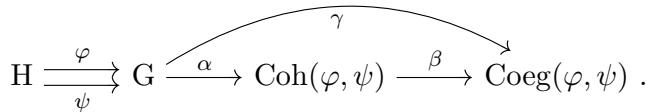
\includegraphics[keepaspectratio]{images/part002_030b7800.jpg}}

在本节（\(n^{o}\)）的余下部分，我们假设偶 \((\varphi,\psi)\) 的框架是一个连通箭图，并固定 G 的一个顶点 \(a_{0}\) 。于是，群胚 \(\mathrm{Coh}(\varphi,\psi)\) 与 \(\mathrm{Coeg}(\varphi,\psi)\) 都是传递的。

以 \(\Gamma\) 表示箭图 \((\mathrm{Som}(\mathrm{G}), \mathrm{Som}(\mathrm{H}), \mathrm{Som}(\varphi), \mathrm{Som}(\psi))\) ，以 \(\widetilde{\Gamma}\) 表示与 \(\Gamma\) 相伴的图，并设 \(\Omega(\widetilde{\Gamma})\) 为有限序列 \((z_1, \ldots, z_n)\) （\(\widetilde{\Gamma}\) 的箭组成的，其中 \(n \geqslant 1\) ）所成的集，这些序列满足：\(z_i\) 的靶是 \(z_{i+1}\) 的起点（若 \(1 \leqslant i < n\) ），且 \(z_n\) 的靶是 \(z_1\) 的起点。在第 1 号中我们构造了一个映射 \(\mathbf{z} \mapsto c(\mathbf{z})\) ，它从集 \(\Omega(\widetilde{\Gamma})\) 映入群 \(\mathrm{Coh}(\varphi, \psi)_{a_0}\) 的共轭类所成的集。

以 \(H \times_{G} H\) 表示 \(H \times H\) 中箭图态射 \(\psi \circ pr_{1}\) 与 \(\varphi \circ pr_{2}\) 的均衡子。其顶点集是 H 的顶点偶 \((a, b)\) （满足 \(\psi(a) = \varphi(b)\) ）所成的集；其箭集是 H 的箭偶 \((f, g)\) （满足 \(\psi(f) = \varphi(g)\) ）所成的集；箭 \((f, g)\) 的起点是顶点 \((o(f), o(g))\) ，其终点是顶点 \((t(f), t(g))\) （参看 II, 第 153 页）。

最后，以 \(\mathrm{Ker}(\varphi, \psi)\) 表示 \(\varphi\) 与 \(\psi\) 的均衡子；回忆（II, 第 165 页, 例 2），这是 H 的子箭图，其顶点 \(a\) 是满足 \(\varphi(a) = \psi(a)\) 的那些顶点，其箭是 \(f \in \mathrm{Fl}(\mathrm{H})\) （满足 \(\varphi(f) = \psi(f)\) ）所成的箭。

命题 4. —— 设 \(\mu\colon\mathrm{H}\times_{\mathrm{G}}\mathrm{H}\to\mathrm{H}\) 为满足 \(\varphi\circ\mu=\varphi\circ\mathrm{pr}_{1}\) 与 \(\psi\circ\mu=\psi\circ\mathrm{pr}_{2}\) 的一个箭图态射。假设：对 H 的每对顶点 \((a,b)\) （满足 \(\varphi(a)=\varphi(b)\) ），存在 H 的一个顶点 \(c\) ，使得 \(\varphi(c)=\psi(b)\) 且 \(a=\mu(b,c)\) 。

  设 \(A_{1}\) 为 \(\mathrm{Ker}(\varphi,\psi)\) 的、与其每个连通分支都相交的顶点集，并设 \(Z_{1}\) 为 \(\Omega(\widetilde{\Gamma})\) 中形如 \(((a,1))\) （其中 \(a\in A_{1}\) ）的元素所成的集。设 \(A_{2}\) 为与 \(H\times_{G}H\) 的每个连通分支都相交的 \(H\times_{G}H\) 的顶点集，并设 \(Z_{2}\) 为形如 \(((a,1),(b,1),(\mu(a,b),-1))\) （其中 \((a,b)\) 取遍 \(A_{2}\) ）的三元组所成的集。

那么，\(\Omega(\widetilde{\Gamma})\) 是 \(\Omega(\widetilde{\Gamma})\) 中包含 \(Z_1 \cup Z_2\) 的最小正规子集。特别地，共轭类 \(c(\mathbf{z})\) （在 \(\mathrm{Coh}(\varphi, \psi)_{a_0}\) 中，其中 \(\mathbf{z}\) 取遍 \(Z_1 \cup Z_2\) ）生成典范同态 \(\beta_{a_0}\) （从 \(\mathrm{Coh}(\varphi, \psi)_{a_0}\) 到 \(\mathrm{Coeg}(\varphi, \psi)_{\beta(a_0)}\) ）的核。

以 \(Z_{1}^{\prime}\) 、\(Z_{2}^{\prime}\) 与 \(Z^{\prime}\) 分别表示 \(\Omega(\widetilde{\Gamma})\) 中包含 \(Z_{1}\) 、\(Z_{2}\) 与 \(Z_{1} \cup Z_{2}\) 的最小正规子集（II, 第 197 页, 定义 1）。目标是证明 \(Z^{\prime}\) 等于 \(\Omega(\widetilde{\Gamma})\) 。由 II, 第 197 页的命题 1 的推论 1（II, 第 199 页），命题的后一断言将由此得出。

引理 1. —— a) 对每个顶点 \(a\) （\(\operatorname{Ker}(\varphi, \psi)\) 的），\(((a, 1))\) 属于 \(Z_1'\) 。

\begin{enumerate}
\def\labelenumi{\alph{enumi})}
\setcounter{enumi}{1}
\item
  对每个顶点 \((a,b)\) （\(\mathrm{H}\times_{\mathrm{G}}\mathrm{H}\) 的），\(((a,1),(b,1),(\mu(a,b),-1))\) 属于 \(\mathbf{Z}_2^{\prime}\) 。
\item
  设 \(A_{1}^{\prime}\) 为顶点 \(a\) （\(\operatorname{Ker}(\varphi,\psi)\) 的，使 \(((a,1))\) 属于 \(Z_{1}^{\prime}\) ）所成的集。我们有 \(A_{1}\subset A_{1}^{\prime}\) （根据 \(Z_{1}^{\prime}\) 的定义）。设 \(f\) 为 \(\operatorname{Ker}(\varphi,\psi)\) 的一条箭，\(a\) 为其起点，\(b\) 为其靶。把正规子集定义中的性质 (iv)（II, 第 197 页, 定义 1）应用于序列 \(((f,1))\) ，便得 \(a\in A_{1}^{\prime}\) 等价于 \(b\in A_{1}^{\prime}\) 。由于 \(A_{1}\) 与 \(\operatorname{Ker}(\varphi,\psi)\) 的每个连通分支相交，我们有 \(A_{1}^{\prime}=\operatorname{Som}(\operatorname{Ker}(\varphi,\psi))\) ，此即所要证明的。
\item
  设 \(A_{2}^{\prime}\) 为顶点 \((a,b)\) （\(H \times_{G} H\) 的，使三元组 \(((a,1),(b,1),(\mu(a,b),-1))\) 属于 \(Z_{2}^{\prime}\) ）所成的集。根据假设，有 \(A_{2} \subset A_{2}^{\prime}\) 。由于 \(A_{2}\) 与 \(H \times_{G} H\) 的每个连通分支相交，只需证明：若存在一条箭 \((f,f^{\prime})\) ，连接顶点 \((a', b')\) 与顶点 \((a, b)\) ，则 \((a, b)\) 属于 \(A_2'\) 当且仅当 \((a', b')\) 亦然。
\end{enumerate}

令 \(f'' = \mu(f, f')\) ；它是一条连接 \(\mu(a', b')\) 与 \(\mu(a, b)\) 的箭，且有 \(\varphi(f'') = \varphi(f)\) 与 \(\psi(f'') = \psi(f')\) 。把 \(\Omega(\widetilde{\Gamma})\) 的正规子集定义中的条件 (iv)（同前）应用于序列 \(((f, 1), (f', 1), (f'', -1))\) ，可知下列两个条件

\begin{enumerate}
\def\labelenumi{(\roman{enumi})}
\item
  三元组 \(((a,1),(b,1),(\mu (a,b), - 1))\) 属于 \(Z^{\prime}\) ；
\item
  三元组 \(((a',1),(b',1),(\mu(a',b'),-1))\) 属于 \(Z'\) 是等价的。这表明 \((a,b)\) 属于 \(A_{2}'\) 当且仅当 \((a',b')\) 属于 \(A_{2}'\) ，引理证明完毕。
\end{enumerate}

我们现在对整数 \(n \geqslant 1\) 作归纳来证明：每个元素 \(((a_1, \varepsilon_1), (a_2, \varepsilon_2), \ldots, (a_n, \varepsilon_n))\) （\(\Omega(\widetilde{\Gamma})\) 的）都属于 \(Z'\) 。

\casehead{\(n = 1\) 的情形}

设 \(((a,\varepsilon))\) 为 \(\Omega(\tilde{\Gamma})\) 的一个长度为 1 的元素。我们有 \(\varphi(a)=\psi(a)\) ，从而 \(((a,1))\in\mathbb{Z}'\)。由引理 1，正规子集定义中的条件 (ii) 进而蕴含 \(((a,-1))\) 属于 \(Z'\) 。

\casehead{\(n \geqslant 2\) 的情形}

根据正规子集的条件 (ii)，只需处理 \(\varepsilon_{2}=1\) 的情形。假设 \(\varepsilon_{1}=1\) ；那么 \((a_{1},a_{2})\) 是 H \(\times_{G}H\) 的一个顶点；令 \(a=\mu(a_{1},a_{2})\) ；由引理 1，三元组 \(((a_{1},1),(a_{2},1),(a,-1))\) 因此属于 \(Z'\)。在 \(\varepsilon_{1}=-1\) 的情形，我们有 \(\varphi(a_{1})=\varphi(a_{2})\) ；因此可以选取 H 的一个顶点 \(a\) ，使得 \(\mu(a_{2},a)=a_{1}\) ，且三元组 \(((a_{2},1),(a,1),(a_{1},-1))\) 属于 \(Z'\) ，于是根据正规子集定义中的条件 (ii)，三元组 \(((a_{1},-1),(a_{2},1),(a,1))\) 也属于 \(Z'\)。

于是，\(((a,\varepsilon_1),(a_3,\varepsilon_3),\ldots ,(a_n,\varepsilon_n))\) 属于 \(\Omega (\widetilde{\Gamma})\) 且长度为 \(n - 1\)。由归纳法，这是 \(\mathbf{Z}'\) 的一个元素。利用正规子集定义中的条件 (i)、(ii) 与 (iii)，我们相继推出下列元素

\[
\begin{array}{c} ((a _ {1}, \varepsilon_ {1}), (a _ {2}, 1), (a, - \varepsilon_ {1}), (a, \varepsilon_ {1}), (a _ {3}, \varepsilon_ {3}), \ldots , (a _ {n}, \varepsilon_ {n})), \\ ((a, - \varepsilon_ {1}), (a, \varepsilon_ {1}), (a _ {3}, \varepsilon_ {3}), \ldots , (a _ {n}, \varepsilon_ {n}), (a _ {1}, \varepsilon_ {1}), (a _ {2}, 1)), \\ ((a _ {3}, \varepsilon_ {3}), \ldots , (a _ {n}, \varepsilon_ {n}), (a _ {1}, \varepsilon_ {1}), (a _ {2}, 1)), \\ ((a _ {1}, \varepsilon_ {1}), (a _ {2}, 1), (a _ {3}, \varepsilon_ {3}), \ldots , (a _ {n}, \varepsilon_ {n})) \end{array}
\]

都属于 Z'。命题证明完毕。

推论. —— a) 采用命题 4 的记号，进一步假设从 Som(H) 映入 Som(G) × Som(G) 的映射 (Som(φ), Som(ψ)) 是单射的，且其像是 Som(G) 上一个等价关系的图。那么，对 H \(\times_{G}\) H 的每个顶点 (a, b)，存在唯一的 H 的顶点 \(c_{a,b}\) ，使得 \(\varphi(c_{a,b}) = \varphi(a)\) 且 \(\psi(c_{a,b}) = \psi(b)\) 。

\begin{enumerate}
\def\labelenumi{\alph{enumi})}
\setcounter{enumi}{1}
\tightlist
\item
  进一步假设：对每条箭 \((f, f')\) （H \(\times_{G}\) H 的），存在 H 的一条箭 \(f''\) ，使得 \(\varphi(f'') = \varphi(f)\) 且 \(\psi(f'') = \psi(f')\) 。
\end{enumerate}

设 A 为与 H \(\times_{G}\) H 的每个连通分支都相交的顶点集。那么，态射 \(\beta_{a_{0}}\) 的核是 \(\mathrm{Coh}(\varphi,\psi)_{a_{0}}\) 中包含共轭类 \(c((a,1),(b,1),(c_{a,b},-1))\) （对 \((a,b)\in\mathrm{A}\) ）的最小正规子群。

设 R 为 \(\operatorname{Som}(\mathrm{G})\) 上以映射 \((\operatorname{Som}(\varphi),\operatorname{Som}(\psi))\) 的像为图的等价关系。设 \((a,b)\) 为 \(H\times_{G}H\) 的一个顶点。于是有 \(\operatorname{R}\{\varphi(a),\psi(a)\}\) 与 \(\operatorname{R}\{\varphi(b),\psi(b)\}\) ，从而 \(\operatorname{R}\{\varphi(a),\psi(b)\}\) （因为 \(\psi(a)=\varphi(b)\) ）。因此，存在唯一的 H 的顶点 \(c\) ，使得 \(\varphi(c)=\varphi(a)\) 且 \(\psi(c)=\psi(b)\) ；把它记作 \(\mu(a,b)\) 。

对每条箭 \((f, f')\) （\(H\times_{G}H\) 的），选取 H 的一条箭 \(f''\) ，使得 \(\varphi(f'') = \varphi(f)\) 且 \(\psi(f'') = \psi(f')\) ，并把它记作 \(\mu(f, f')\) 。

我们就这样定义了一个箭图态射 \(\mu\colon\mathrm{H}\times_{\mathrm{G}}\mathrm{H}\to\mathrm{H}\) ，满足 \(\varphi\circ\mu=\varphi\circ\mathrm{pr}_{1}\) 与 \(\psi\circ\mu=\psi\circ\mathrm{pr}_{2}\) 。

设 \((a,b)\) 为满足 \(\varphi(a)=\varphi(b)\) 的一对 H 的顶点。我们有 \(\mathrm{R}\{\varphi(a),\psi(a)\}\) 与 \(\mathrm{R}\{\varphi(b),\psi(b)\}\) ，因此 \(\mathrm{R}\{\psi(b),\psi(a)\}\) 。从而存在唯一的 H 的顶点 \(c\) ，使得 \(\varphi(c)=\psi(b)\) 且 \(\psi(c)=\psi(a)\) 。顶点 \(\mu(b,c)\) 满足 \(\varphi(\mu(b,c))=\varphi(b)=\varphi(a)\) 与 \(\psi(\mu(b,c))=\psi(c)=\psi(a)\) 。 我们因此有 \(\mu(b,c)=a\) ，因为映射 \((\operatorname{Som}(\varphi),\operatorname{Som}(\psi))\) （从 \(\operatorname{Som}(\operatorname{H})\) 映入 \(\operatorname{Som}(\operatorname{G})\times\operatorname{Som}(\operatorname{G})\) ）是单射的。

设 \(A_{1}\) 为 \(\operatorname{Ker}(\varphi,\psi)\) 的顶点集，并设 \(Z_{1}\) 为 \(\Omega(\widetilde{\Gamma})\) 中形如 \(((a,1))\) （对 \(a\in A_{1}\) ）的元素所成的集。令 \(A_{2}=A\) ，并设 \(Z_{2}\) 为形如 \(((a,1),(b,1),(\mu(a,b),-1))\) 的元素（\(\Omega(\widetilde{\Gamma})\) 的，对 \((a,b)\in A_{2}\) ）所成的集。以 \(\widetilde{Z}\) （相应地 \(\widetilde{Z}_{1}\) ，或 \(\widetilde{Z}_{2}\)）表示 \(\Omega(\widetilde{\Gamma})\) 中包含 \(Z_{1}\cup Z_{2}\) （相应地 \(Z_{1}\) ，或 \(Z_{2}\)）的最小正规子集。

设 \(a \in \mathrm{A}_1\) 。我们有 \(\varphi(a) = \psi(a)\) ；令 \(x = \varphi(a)\)。顶点 \(a\) 是满足 \(\varphi(a) = \psi(a) = x\) 的 H 的唯一顶点。特别地，我们有 \(\mu(a, a) = a\)。因此三元组 \(((a, 1), (a, 1), (a, -1))\) 属于 \(\mathbf{Z}_2\)。进而由正规子集定义中的条件 (i) 与 (iii) 得出 \(((a, 1))\) 属于 \(\widetilde{\mathbf{Z}}_2\)。从而我们有 \(\mathbf{Z}_1 \subset \widetilde{\mathbf{Z}}_2\) ，于是 \(\widetilde{\mathbf{Z}} = \widetilde{\mathbf{Z}}_2\) 。

由命题 4，\(\Omega(\tilde{\Gamma})\) 是 \(\Omega(\tilde{\Gamma})\) 中包含 \(Z_{2}\) 的最小正规子集，且 \(\beta_{a_{0}}\) 的核是 \(\mathrm{Coh}(\varphi,\psi)_{a_{0}}\) 中包含共轭类 \(c(\mathbf{z})\) （对 \(\mathbf{z}\in Z_{2}\) ）的最小正规子群。推论得证。

例. —— 设 X 与 R 为拓扑空间，o 与 t 为从 R 到 X 的连续映射，C 为偶 \((f,g)\in\mathrm{R}^{2}\) （满足 \(t(f)=o(g)\) ）所成的集，m 为使箭图 \((\mathrm{X},\mathrm{R},o,t)\) 成为一个群胚的从 C 到 R 的连续映射；进一步假设从 R 到 R 的映射 \(f\mapsto f^{-1}\) 是连续的。若令 \(\mathrm{H}=\varpi(\mathrm{R})\) 、\(\mathrm{G}=\varpi(\mathrm{X})\) 、\(\varphi=\varpi(o)\) 、\(\psi=\varpi(t)\) 与 \(\mu=\varpi(m)\) ，则命题的假设得到满足。

进一步假设 R 是 X 上一个等价关系的图，其中映射 o 与 t 由 \(X \times X\) 到 X 的投影通过取子空间导出。于是推论的假设得到满足。

注记. —— *更一般地，当 (G, H, \(\varphi\) , \(\psi\) , \(\mu\) ) 是一个“群胚的群胚”时，命题的假设得到满足。这意味着 G 与 H 都是群胚，\(\varphi\) 与 \(\psi\) 是从 H 到 G 的群胚态射，使四元组 (G, H, \(\varphi\) , \(\psi\) ) 成为一个“群胚箭图”；最后，\(\mu\) 是这个“箭图”中由一个群胚态射 H \(\times_{\mathrm{G}}\) H → H 给出的合成法则，它满足表达该法则的结合性以及每条“箭”皆可逆的一定数目的性质。读者还会注意到，本书中所研究的基本群胚的应用全都属于这种情形。

\subsection{余均衡子的迷向群}

设 G 与 H 为群胚；设 \(\varphi\) 与 \(\psi\) 为从 H 到 G 的群胚态射。本节的目的在于总结上同伦子的迷向群的计算（II, 第 193 页, 命题 6）以及上一节中所作的上同伦子与余均衡子的迷向群的比较，以便由此推出余均衡子 Coeg( \(\varphi\) , \(\psi\) ) 的迷向群的计算。

以 \(\alpha\colon\mathrm{G}\to\mathrm{Coh}(\varphi,\psi)\) 、\(\beta\colon\mathrm{Coh}(\varphi,\psi)\to\mathrm{Coeg}(\varphi,\psi)\) 与 \(\gamma=\beta\circ\alpha\colon\mathrm{G}\to\mathrm{Coeg}(\varphi,\psi)\) 表示典范群胚态射。以 \(h\colon\mathrm{Som}(\mathrm{H})\to\mathrm{Fl}(\mathrm{Coh}(\varphi,\psi))\) 表示典范同伦；回忆 \(\mathrm{Coh}(\varphi,\psi)\) 的顶点集等于 \(\mathrm{Som}(\mathrm{G})\) 。

以 \(\Gamma\) 表示箭图 (Som(G), Som(H), Som(φ), Som(ψ))，再以 \(\varphi_0\) 与 \(\psi_0\) 表示由 \(\varphi\) 与 \(\psi\) 通过取轨道诱导的映射，以 \(\Gamma_0\) 表示 (Orb(G), Orb(H), \(\varphi_0, \psi_0\) ) ，即偶 ( \(\varphi, \psi\) ) 的框架。我们将假设箭图 \(\Gamma_0\) 是连通的且其顶点集非空，这等价于假设群胚 Coh(φ, ψ) 与 Coeg(φ, ψ) 都是传递的。

回忆（参看 II, 第 192 页, 定义 4），基本配备由下列数据组成：一个族 \((a, b, c_1, c_2, \mathrm{T}, i_0)\) ，其中：对所有 \(i \in \mathrm{Orb}(\mathrm{G})\) ，\(a(i)\) 是轨道 \(i\) （\(\mathrm{G}\) 的）中的一个顶点；对每个 \(j \in \mathrm{Orb}(\mathrm{H})\) ，\(b(j)\) 是轨道 \(j\) （\(\mathrm{H}\) 的）中的一个顶点，\(c_1(j)\) 与 \(c_2(j)\) 分别是 \(\mathrm{G}\) 中从 \(\varphi(b(j))\) 到 \(a(\varphi_0(j))\) 以及从 \(\psi(b(j))\) 到 \(a(\psi_0(j))\) 的箭；\(\mathrm{T}\) 是 \(\Gamma_0\) 的一个子箭图，其相伴树是图 \(\widetilde{\Gamma}_0\) 的一个极大树；最后，\(i_0\) 是 \(\mathrm{G}\) 的一个轨道，且我们令 \(a_0 = a(i_0)\) 。

我们随后定义一个箭图态射 \(\tau_0\) （从 \(\Gamma_0\) 到 \(\mathrm{Coh}(\varphi, \psi)\) ），使得 \(\tau_0(i) = \beta(a(i))\) 以及 \(\tau_0(j) = \alpha(c_1(j))^{-1}h(b(j))\alpha(c_2(j))\) （对 \(i \in \mathrm{Orb}(\mathrm{G})\) 及 \(j \in \mathrm{Orb}(\mathrm{H})\) ）。若 \(i\) 属于 \(\mathrm{Orb}(\mathrm{G})\) ，设 \(d_i\) 为图 \(\widetilde{\mathrm{T}}\) 中连接 \(i_0\) 与 \(i\) 的唯一的道路类，并以 \(\delta_i\) 表示它在 \(\mathrm{Coh}(\varphi, \psi)\) 中的、由群胚态射 \(\tau_0\) 给出的像。

由这些数据，II, 第 193 页的命题 6 给出一个满射同态。

\[
\Lambda \colon \bigl (\underset {i \in \pi_ {0} (\mathrm{G})} {*} \mathrm{G} _ {a (i)} \bigr) * \mathrm{F} (\operatorname{Orb} (\mathrm{H})) \to \operatorname{Coh} (\varphi , \psi) _ {a (i _ {0})}
\]

并描述其核的生成元，从而给出群 \(\mathrm{Coh}(\varphi,\psi)_{a_{0}}\) 的一个表现。

长度 \(\geqslant 1\) 的回路所成的集——在图 \(\widetilde{\Gamma}\) （与 \(\Gamma\) 相伴的）中——与集 \(\Omega(\widetilde{\Gamma})\) ——即序列 \((z_1, \ldots, z_n)\) （\(\widetilde{\Gamma}\) 的箭组成的，以 \(\mathbf{Z}/n\mathbf{Z}\) 为指标集）所成的集——等同，其中 \(n\) 取遍整数集 \(\geqslant 1\) ，且对每个 \(k \in \mathbf{Z}/n\mathbf{Z}\) ，\(z_k\) 的靶是 \(z_{k+1}\) 的起点。设 \(\mathbf{Z}\) 为 \(\Omega(\widetilde{\Gamma})\) 的一个子集，使共轭类 \(c(z)\) （对 \(z \in \mathbf{Z}\) ）生成满射同态 \(\beta_{a_0}\) 的核。同态 \(\beta_{a_0} \circ \Lambda\) 是满射的；为由此推出它的核，即群 \(\operatorname{Coeg}(\varphi, \psi)_{\beta(a_0)}\) 的一个表现，还需对每个 \(z \in \mathbf{Z}\) 选取一个元素 \(\mathrm{C}(z)\) （在群 \(\left( \begin{array}{cc} * & \mathrm{G}_{a(i)} \\ i \in \mathrm{Orb}(\mathrm{G}) & \end{array} \right) * \mathrm{F}(\pi_0(\mathrm{H}))\) 中），使 \(\Lambda(\mathrm{C}(z))\) 属于共轭类 \(c(z)\) 。

于是设 \(z = (z_{1}, \ldots, z_{n})\) 为 \(\Omega(\tilde{\Gamma})\) 的一个元素；令 \(z_{k} = (y_{k}, \varepsilon_{k})\) ，其中 \(y_{k} \in \mathrm{Fl}(\Gamma) = \mathrm{Som}(\mathrm{H})\) 且 \(\varepsilon_{k} \in \{\pm 1\}\) 。根据定义，\(c(z)\) 是元素的共轭类

\[
g h (y _ {1}) ^ {\varepsilon_ {1}} \dots h (y _ {n}) ^ {\varepsilon_ {n}} g ^ {- 1}
\]

的、在群 \(\mathrm{Coh}(\varphi,\psi)_{a_{0}}\) 中的共轭类，其中 g 是 \(\mathrm{Coh}(\varphi,\psi)\) 中连接 \(a_{0}\) 与 \(z_{1}\) 的起点的任意一条箭。对 \(k \in Z/nZ\) ，设 \(j_{k}\) 为 \(y_{k}\) 在 H 中的轨道，并选取 H 的一条箭 \(f_{k}\) ，它连接 \(y_{k}\) 与顶点 \(b(j_{k})\)。根据同伦的定义，我们随后有关系式

\[
h (y _ {k}) (\alpha \circ \psi) (f _ {k}) = (\alpha \circ \varphi) (f _ {k}) h (b (j _ {k}))
\]

在群胚 \(\mathrm{Coh}(\varphi,\psi)\) 中成立。于是，利用箭图态射 \(\tau_{0}\) 的定义，我们有

\[
\begin{array}{l} h (y _ {k}) = (\alpha \circ \varphi) (f _ {k}) \cdot h (b (j _ {k})) \cdot (\alpha \circ \psi) (f _ {k}) ^ {- 1} \\ \quad = (\alpha \circ \varphi) (f _ {k}) \cdot (\alpha \circ c _ {1}) (j _ {k}) \cdot \tau_ {0} (j _ {k}) \cdot (\alpha \circ c _ {2}) (j _ {k}) ^ {- 1} \cdot (\alpha \circ \psi) (f _ {k}) ^ {- 1} \\ \quad = (\alpha \circ \varphi) (f _ {k}) \cdot (\alpha \circ c _ {1}) (j _ {k}) \cdot \delta_ {\varphi_ {0} (j _ {k})} ^ {- 1} \cdot \\ \quad \cdot \delta_ {\varphi_ {0} (j _ {k})} \cdot \tau_ {0} (j _ {k}) \cdot \delta_ {\psi_ {0} (j _ {k})} ^ {- 1} \cdot \\ \quad \cdot \delta_ {\psi_ {0} (j _ {k})} \cdot (\alpha \circ c _ {2}) (j _ {k}) ^ {- 1} \cdot (\alpha \circ \psi) (f _ {k}) ^ {- 1} \\ = u _ {k} \Lambda (j _ {k}) v _ {k}, \end{array}
\]

其中我们已令

\[
u _ {k} = \alpha (\varphi (f _ {k}) c _ {1} (j _ {k})) \cdot \delta_ {\varphi_ {0} (j _ {k})} ^ {- 1} \quad \text { and } \quad v _ {k} = \delta_ {\psi_ {0} (j _ {k})} \cdot \alpha (\psi (f _ {k}) c _ {2} (j _ {k})) ^ {- 1}.
\]

对每个元素 \(k \in \mathbf{Z}/n\mathbf{Z}\) ，定义箭 \(\widetilde{u}_{k}, \widetilde{v}_{k}\) （G 中的）如下

\[
h (y _ {k}) ^ {\varepsilon_ {k}} = \widetilde {u} _ {k} \Lambda (j _ {k}) ^ {\varepsilon_ {k}} \widetilde {v} _ {k},
\]

使得

\[
(\widetilde {u} _ {k}, \widetilde {v} _ {k}) = \left\{ \begin{array}{l l} (u _ {k}, v _ {k}) & \text { if } \varepsilon_ {k} = 1; \\ (v _ {k} ^ {- 1}, u _ {k} ^ {- 1}) & \text { if } \varepsilon_ {k} = - 1. \end{array} \right.
\]

以 \(x_{k}\) 表示箭 \(h(y_{k})^{\varepsilon_{k}}\) 的起点；其靶则为 \(x_{k+1}\) ；设 \(i_{k}\) 为 \(x_{k}\) 的轨道。于是我们用下列公式定义群胚 G 中的回路 \(\lambda_{k}(z)\) （以 \(a(i_{k})\) 为基点的）：

\[
\lambda_ {k} (z) = \left\{ \begin{array}{l l} c _ {2} (j _ {k - 1}) ^ {- 1} \psi (f _ {k - 1}) ^ {- 1} \varphi (f _ {k}) c _ {1} (j _ {k}) & \text {if} (\varepsilon_ {k - 1}, \varepsilon_ {k}) = (1, 1); \\ c _ {2} (j _ {k - 1}) ^ {- 1} \psi (f _ {k - 1}) ^ {- 1} \psi (f _ {k}) c _ {2} (j _ {k}) & \text {if} (\varepsilon_ {k - 1}, \varepsilon_ {k}) = (1, - 1); \\ c _ {1} (j _ {k - 1}) ^ {- 1} \varphi (f _ {k - 1}) ^ {- 1} \varphi (f _ {k}) c _ {1} (j _ {k}) & \text {if} (\varepsilon_ {k - 1}, \varepsilon_ {k}) = (- 1, 1); \\ c _ {1} (j _ {k - 1}) ^ {- 1} \varphi (f _ {k - 1}) ^ {- 1} \psi (f _ {k}) c _ {2} (j _ {k}) & \text {if} (\varepsilon_ {k - 1}, \varepsilon_ {k}) = (- 1, - 1) \end{array} \right.\tag{1}
\]

根据构造，我们有

\[
\Lambda (\lambda_ {k} (z)) = \widetilde {v} _ {k - 1} \widetilde {u} _ {k},
\]

从而元素在同态 \(\Lambda\) 下的像

\[
\mathrm{C} (z) = \lambda_ {1} (z) (j _ {1}) ^ {\varepsilon_ {1}} \lambda_ {2} (z) (j _ {2}) ^ {\varepsilon_ {2}} \dots \lambda_ {n} (z) (j _ {n}) ^ {\varepsilon_ {n}}\tag{2}
\]

属于共轭类 \(c(z)\) 。

定义 3. —— 设 G 与 H 为群胚；设 \(\varphi\) 与 \(\psi\) 为从 H 到 G 的群胚态射。我们假设群胚 Coeg \((\varphi, \psi)\) 是传递的。设 \((a, b, c_1, c_2, T, i_0)\) 为偶 \((\varphi, \psi)\) 的一个基本配备。

我们称补配备为下列数据：一个子集 Z （\(\Omega(\widetilde{\Gamma})\) 的），使共轭类 \(c(\mathbf{z})\) （对 \(\mathbf{z} \in \mathbf{Z}\) ）生成同态 \(\beta_{a(i_0)}\) 的核；并且，对 Z 的每个元素 \(\mathbf{z} = ((y_1, \varepsilon_1), \ldots, (y_n, \varepsilon_n))\) ，给出箭的一个序列 \(f(\mathbf{z}) = (f_1, \ldots, f_n)\) （H 中的），使得 \(f_k\) 连接 \(y_k\) 与顶点 \(b(j_k)\) ，其中 \(j_k\) 表示 \(y_k\) 在 H 中的轨道。

偶 \((\varphi,\psi)\) 的一个完备配备是指一个基本配备与一个补配备的数据。

命题 5. —— 设 G 与 H 为群胚；设 \(\varphi\) 与 \(\psi\) 为从 H 到 G 的群胚态射。假设群胚 \(\operatorname{Coeg}(\varphi, \psi)\) 是传递的。以 \(\gamma\colon \mathrm{G} \to \mathrm{Coeg}(\varphi, \psi)\) 表示典范群胚态射。

我们给偶 \((\varphi, \psi)\) 配备一个完备配备

\[
(a, b, c _ {1}, c _ {2}, \mathrm{T}, i _ {0}, \mathrm{Z}, (f (\mathbf {z})) _ {\mathbf {z} \in \mathrm{Z}}).
\]

对 \(j \in \text{Orb(H)}\) ，设 \(\varphi_j \colon \text{H}_{b(j)} \to \text{G}_{a(\varphi_0(j))}\) 与 \(\psi_j \colon \text{H}_{b(j)} \to \text{G}_{a(\psi_0(j))}\) 分别为群同态 \(\text{Int}(c_1(j))^{-1} \circ \varphi_{b(j)}\) 与 \(\text{Int}(c_2(j))^{-1} \circ \psi_{b(j)}\) ，其中 \(\varphi_0\) 与 \(\psi_0\) 表示由 \(\varphi\) 与 \(\psi\) 通过取轨道诱导的典范映射。设 \(\tau\) 为框架 \(\Gamma_0\) （偶 \((\varphi, \psi)\) 的）到 \(\text{Coeg}(\varphi, \psi)\) 中的态射，由 \(\text{Som}(\tau)(i) = \gamma(a(i))\) （若 \(i \in \text{Orb(G)}\) ）定义，且使 \(\text{Fl}(\tau)(j)\) 是道路 \(\gamma(c_1(j))^{-1} \gamma(c_2(j))\) （在 \(\text{Coeg}(\varphi, \psi)\) 中的）。若 \(i\) 是 G 的一个轨道，设 \(c_i\) 为 \(\widetilde{\text{T}}\) 中连接 \(i_0\) 与 \(i\) 的唯一的道路类，并令 \(\delta_i = \widetilde{\tau}(c_i)\) ，其中 \(\widetilde{\tau} \colon \text{Grp(G)} \to \text{Coeg}(\varphi, \psi)\) 是由 \(\tau\) 诱导的典范群胚态射。

于是存在唯一的群同态

\[
\lambda \colon \bigl ( \begin{array}{c} * \\ i \in \operatorname{Orb} (\mathrm{G}) \end{array} \mathrm{G} _ {a (i)} \bigr) * \mathrm{F} (\operatorname{Orb} (\mathrm{H})) \to \operatorname{Coeg} (\varphi , \psi) _ {\gamma (a (i _ {0}))}
\]

使得

\[
\begin{array}{l l} \lambda (f) = \delta_ {i} \gamma_ {a (i)} (f) \delta_ {i} ^ {- 1} & \text { for } i \in \mathrm{Orb(G)} \text { and } f \in \mathrm{G} _ {a (i)}, \\ \lambda (j) = \delta_ {\varphi_ {0} (j)} \tau (j) \delta_ {\psi_ {0} (j)} ^ {- 1} & \text { for } j \in \mathrm{Orb(H)}. \end{array}
\]

同态 \(\lambda\) 是满射的；其核是包含下列元素的最小正规子群：

\[
\left(\mathrm{R} _ {1}\right) \quad r _ {1} (j) = j \quad \text { for } j \text { in } \mathrm{Fl} (\mathrm{T});
\]

\[
(\mathrm{R} _ {2}) \quad r _ {2} (j, f) = \varphi_ {j} (f) j \psi_ {j} (f) ^ {- 1} j ^ {- 1}
\]

\[
\text { for } j \in \operatorname{Orb} (\mathrm{H}) \text { and } f \in \mathrm{H} _ {b (j)};\tag{\((R_{3})\)}
\]

\[
r _ {3} (z) = \lambda_ {1} (z) j _ {1} ^ {\varepsilon_ {1}} \lambda_ {2} (z) j _ {2} ^ {\varepsilon_ {2}} \dots \lambda_ {n} (z) j _ {n} ^ {\varepsilon_ {n}}
\]

\[
\text { for } z = ((y _ {1}, \varepsilon_ {1}), \dots , (y _ {n}, \varepsilon_ {n})) \in \mathbf {Z},
\]

其中回路 \(\lambda_{i}(z)\) 由第 208 页的公式 (1) 定义。

这样一个态射的存在性与唯一性由群的族的自由积的泛性质得出（A, I, 第 85 页, 命题 8）。以 \(\alpha\colon G\to\mathrm{Coh}(\varphi,\psi)\) 与 \(\beta\colon\mathrm{Coh}(\varphi,\psi)\to\mathrm{Coeg}(\varphi,\psi)\) 表示典范态射，于是 \(\gamma=\beta\circ\alpha\)。再设 \(h\colon\mathrm{Som}(H)\to\mathrm{Fl}(\mathrm{Coh}(\varphi,\psi))\) 为联系 \(\alpha\circ\varphi\) 与 \(\alpha\circ\psi\) 的典范同伦。由于 \(\beta\) 是通过缩并 \(h\) 的像中的箭而得到的群胚态射，我们有

\[
\operatorname{Fl} (\tau) (j) = \gamma (c _ {1} (j)) ^ {- 1} \gamma (c _ {2} (j)) = \gamma (c _ {1} (j) ^ {- 1}) \beta (h (j)) \gamma (c _ {2} (j)) = \beta (\tau_ {0} (j))
\]

在 \(\operatorname{Coeg}(\varphi,\psi)\) 中成立，其中 \(\tau_{0}\colon\Gamma_{0}\to\mathrm{Coh}(\varphi,\psi)\) 表示由基本配备 \((a,b,c_{1},c_{2},\mathrm{T},i_{0})\) 诱导的箭图态射。于是，同态 \(\lambda\) 是命题 6（II, 第 193 页）中所定义的同态 \(\Lambda\) 与满射同态 \(\beta_{a(i_0)}\) 的复合。它特别是满射的。

设 \(z \in \mathbf{Z}\)。根据构造，\(\Lambda(r_3(z))\) 属于共轭类 \(c(z)\) 。根据补配备的定义，同态 \(\beta_{a(i_0)}\) 的核因此是 \(\mathrm{Coh}(\varphi, \psi)_{a(i_0)}\) 中包含元素 \(\Lambda(r_3(z))\) （对 \(z \in \mathbf{Z}\) ）的最小正规子群。由于同态 \(\Lambda\) 是满射的，同态 \(\lambda = \beta_{a(i_0)} \circ \Lambda\) 的核因此是群 \(\left( *_{i \in \mathrm{Orb}(G)} G_{a(i)} \right) * F(\pi_0(H))\) 中包含 \(\Lambda\) 的核的、由公式 \((R_1), (R_2)\) 给出的生成元以及由公式 \((R_3)\) 定义的元素的最小正规子群。命题得证。

\subsection{群胚被群作用的商}

设 G 为一个传递群胚，K 为一个群，并设 \(\theta\colon\mathrm{K}\to\mathrm{Aut}(\mathrm{G})^{\circ}\) 为从 K 到群胚 G 的自同构群之相反群中的群同态。我们将说群 K 右作用于 G。若 \(k\in\mathrm{K}\) ，我们有时以 \(k^{*}x\) （相应地 \(k^{*}f\) ）表示 G 的顶点 \(x\) （相应地箭 \(f\) ）在群胚自同构 \(\theta(k)\) 下的像。

设 \(|\mathrm{K}|\) 为这样的群胚：其顶点集为 \(\mathrm{K}\) ，连接两个顶点的箭集当这两个顶点不同时为空集，否则缩为单个元素。设 \(\mathrm{H}\) 为积群胚 \(\mathrm{G} \times |\mathrm{K}|\) ；\(\mathrm{H}\) 的一个顶点是偶 \((a,k)\) ，其中 \(a\) 是 \(\mathrm{G}\) 的一个顶点，\(k\) 是 \(\mathrm{K}\) 的一个元素；若 \(f\) 是 \(\mathrm{G}\) 中连接顶点 \(a\) 与顶点 \(b\) 的一条箭，我们以 \((f,k)\) 表示 \(\mathrm{H}\) 中连接 \((a,k)\) 与 \((b,k)\) 的唯一的箭。设 \(\varphi: \mathrm{H} \to \mathrm{G}\) 为由第一个投影给出的群胚态射，并设 \(\psi: \mathrm{H} \to \mathrm{G}\) 为满足 \(\operatorname{Som}(\psi)((a,k)) = k^*a\) 与 \(\operatorname{Fl}(\psi)((f,k)) = k^*f\) （若 \(k \in \mathrm{K}\) 、\(a \in \operatorname{Som}(\mathrm{G})\) 且 \(f \in \operatorname{Fl}(\mathrm{G})\) ）的群胚态射。

以 G/K 表示余均衡子 \(\operatorname{Coeg}(\varphi,\psi)\) ，并以 \(\gamma\colon G\to G/K\) 表示典范群胚态射。

设 o 为 G 的一个顶点。对 \(k \in K\) ，选取 G 中的一条箭 \(c_{k}\) （连接 \(k^{*}o\) 与 o 的）；由于 G 是传递的，这样的箭存在。对 \(k \in K\) ，以 \(\text{Fix}(k)\) 表示 G 的子群胚，其顶点（相应地箭）是被 k 固定的 \(\text{Som}(G)\) （相应地 \(\text{Fl}(G)\) ）的元素；我们选取一个顶点集 \(A_{k}\) （\(\text{Fix}(k)\) 的，与此群胚的所有轨道都相交）。对 \(k \in K\) 及 \(a \in A_{k}\) ，我们还选取 G 中连接顶点 a 与顶点 o 的一条箭 \(f_{(a,k)}\) 。

命题 6. —— 唯一的群同态

\[
\lambda \colon \mathrm{G} _ {o} * \mathrm{F} (\mathrm{K}) \to (\mathrm{G} / \mathrm{K}) _ {\gamma (o)}
\]

使得 \(\lambda(f) = \gamma_o(f)\) （对 \(f \in \mathrm{G}_o\) ）以及 \(\lambda([k]) = \gamma(c_k)\) （对 \(k \in \mathrm{K}\) ）者是满射的。其核是 \(\mathrm{G}_o * \mathrm{F}(\mathrm{K})\) 中包含下列元素的最小正规子群：

\[
r _ {2} (k, f) = [ k ] ^ {- 1} f [ k ] (c _ {k} ^ {- 1} k ^ {*} (f) ^ {- 1} c _ {k})\tag{\((R_{2})\)}
\]

\[
\text { for } k \in \mathrm{K} \text { and } f \in \mathrm{G} _ {o};\tag{\((\mathrm{R}_{3}^{\prime})\)}
\]

\[
r _ {3} ^ {\prime} (k, a) = [ k ] (c _ {k} ^ {- 1} k ^ {*} (f _ {(a, k)}) ^ {- 1} f _ {(a, k)}))
\]

\[
\text { for } k \in \mathrm{K} - \{e \} \text { and } a \in \mathrm{A} _{k}\tag{\((\mathrm{R}_{3}^{\prime\prime})\)}
\]

\[
r _ {3} ^ {\prime \prime} (k, h) = [ k h ] ^ {- 1} [ k ] [ h ] (c _ {h} ^ {- 1} h ^ {*} (c _ {k} ^ {- 1}) c _ {k h})
\]

\[
\text { for } k,h \in \mathrm{K}.
\]

由于 G 是传递的，把元素 \(k \in K\) 对应到 \((o, k)\) 的轨道的映射是 K 到 H 的轨道集上的一个双射。我们于是把 \(\operatorname{Orb}(\mathbf{G})\) 与 \(\{o\}\) 等同，把 \(\operatorname{Orb}(\mathbf{H})\) 与 K 等同。框架 \(\Gamma_{0}\) （偶 \((\varphi, \psi)\) 的）于是等同于具有单个顶点 o 且箭集为 K 的箭图。设 T 为 \(\Gamma_{0}\) 的、顶点集为 \(\{o\}\) 而箭集为空的子箭图；其相伴图是图 \(\widetilde{\Gamma}_{0}\) 的唯一的极大树。

族 \((o,(o,k)_{k\in \mathrm{K}},(e_o)_{k\in \mathrm{K}},(c_k)_{k\in \mathrm{K}},\mathrm{T},o)\) 是偶 \((\varphi ,\psi)\) 的一个基本配备。

映射 \(f \mapsto (f, k)\) 定义了迷向群 \(G_o\) 到迷向群 \(H_{(o,k)}\) 上的一个同构；在此同构下，同态 \(\varphi_k\) 与 \(\psi_k\) （从 \(H_{(o,k)}\) 到 \(G_o\) 中的、由 II, 第 208 页的命题 5 定义的）由下式给出

\[
\varphi_ {k} (f, k) = f \quad \text { and } \quad \psi_ {k} (f, k) = c _ {k} ^ {- 1} k ^ {*} (f) c _ {k},\tag{3}
\]

（对 \(k\in \mathrm{K}\) 及 \(f\in \mathrm{G}_o\) ）。

箭图 \(H \times_{G} H\) 是 \(H \times H\) 中箭图态射 \(\psi \circ pr_{1}\) 与 \(\varphi \circ pr_{2}\) 的均衡子。其顶点是偶 \(((a, k), (b, h))\) ，其中 a 与 b 是 G 的顶点，k 与 h 是 K 中满足 \(b = k^{*}a\) 的元素；其箭是偶 \(((f, k), (g, h))\) ，其中 f 与 g 是 G 的箭，k 与 h 是 K 中满足 \(g = k^{*}f\) 的元素；箭 \(((f,k),(g,h))\) 的起点等于 \(((o(f),k),(o(g),h))\) ；其靶等于 \(((t(f),k),(t(g),h))\) 。

我们随后定义一个箭图态射 \(\mu\) （从 \(H \times_{\mathrm{G}} H\) 到 H 中的），令 \(\mu((a,k),(b,h)) = (a,kh)\) 与 \(\mu((f,k),(g,h)) = (f,kh)\) 。我们有 \(\varphi \circ \mu = \varphi \circ \mathrm{pr}_1\) 与 \(\psi \circ \mu = \psi \circ \mathrm{pr}_2\) 。

设 \(x\) 与 \(y\) 为 H 中满足 \(\varphi(x) = \varphi(y)\) 的顶点。于是存在 G 的一个顶点 \(a\) 以及 K 的元素 \(k\) 与 \(h\) ，使得 \(x = (a, k)\) 且 \(y = (a, h)\) 。令 \(z = (h^* a, h^{-1} k)\) ；我们有 \(\mu(y, z) = x\)。这表明偶 \((\varphi, \psi)\) 满足 II, 第 202 页的命题 4 的假设。

H 的顶点 \((a,k)\) 属于群胚 \(\operatorname{Ker}(\varphi,\psi)\) （\(\varphi\) 与 \(\psi\) 的均衡子）当且仅当 \(k^{*}a=a\) ，即 k 属于群 K 中顶点 a 的稳定子。设 \(A_{1}\) 为偶 \((a,k)\) （对 \(k\in K\) 与 \(a\in A_{k}\)）所成的集；它与 H 的子群胚 \(\operatorname{Ker}(\varphi,\psi)\) 的所有轨道相交。设 \(Z_{1}\) 为 \(\Omega(\widetilde{\Gamma})\) 中由形如 (((a,k),1)) （对 \((a,k)\in A_{1}\)）的序列组成的部分。对 \(\mathbf{z}=((a,k),1)\in\mathbf{Z}_{1}\) ，\((f_{(a,k)},k)\) 是 H 的一条箭，它连接 \((a,k)\) 与 \((o,k)\) 。令 \(f(\mathbf{z})=((f_{(a,k)},k))\)。

顶点所成的集 \(\mathrm{A}_2\) （\(\mathrm{H} \times_{\mathrm{G}} \mathrm{H}\) 的，由形如 \(((o,k), (k^*o,h))\) （对 \((k,h) \in \mathrm{K}^2\) ）的顶点组成）与 \(\mathrm{H} \times_{\mathrm{G}} \mathrm{H}\) 的每个轨道相交。还可注意到 \(\mu((o,k), (k^*o,h)) = (o,kh)\) 。H 中的箭 \((e_o,k), (c_k,h), (e_o,kh)\) 分别连接 \((o,k), (k^*o,h), (o,kh)\) 到 \((o,k), (o,h)\) 与 \((o,kh)\) 。以 \(\mathrm{Z}_2\) 表示形如 \((((o,k),1), ((k^*o,h), 1), ((o,kh), -1))\) 的序列在 \(\Omega(\widetilde{\Gamma})\) 中所成的集；对这样一个元素 \(\mathbf{z}\) （\(\mathrm{Z}_2\) 的），令 \(f(\mathbf{z}) = ((e_o,k), (c_k,h), (e_o,kh))\) 。

由 II, 第 202 页的命题 4，集 \(Z = Z_1 \cup Z_2\) 与族 \((f(\mathbf{z}))_{z \in \mathbb{Z}}\) 构成一个补配备。

设 \(k \in \mathrm{K}\) 且 \(a \in \mathrm{A}_k\) 。元素 \(\mathrm{C}((a, k), 1)\) （由 II, 第 208 页的公式 (2) 定义的、群 \(\mathrm{G}_o * \mathrm{F}(\mathrm{K})\) 中的）等于

\[
c _ {k} ^ {- 1} \psi ((f _ {(a, k)}, k)) ^ {- 1} \varphi (f _ {(a, k)}) e _ {o} [ k ] = (c _ {k} ^ {- 1} k ^ {*} (f _ {(a, k)}) ^ {- 1} f _ {(a, k)}) [ k ].\tag{4}
\]

设 \(k,h \in \mathbf{K}\)。我们验证，元素

\[
\mathrm{C} (((o, k), 1), ((k ^ {*} o, h), 1), ((o, k h), - 1))
\]

（由 II, 第 208 页的公式 (2) 定义的、群 \(G_{o} * F(K)\) 中的）等于

\[
[ k ] [ h ] (c _ {h} ^ {- 1} h ^ {*} (c _ {k} ^ {- 1}) c _ {k h}) [ k h ] ^ {- 1}.\tag{5}
\]

元素 \(r_3'(e, a)\) （由关系式 \((\mathrm{R}_3')\) 对 \(k = e\) 给出的）都等于 \([e]c_e^{-1}\) ，后者是群 \(\mathrm{G}_o * \mathrm{F}(\mathrm{K})\) 中把关系式 \((\mathrm{R}_{3}^{\prime\prime})\) 应用于 \(k = h = e\) 而得到的元素。鉴于关系式 (3)、(4) 与 (5)，命题于是由 II, 第 208 页, 命题 5 得出。

推论 1. —— 假设群 K 由 G 的顶点的固定子生成。那么群同态 \(\gamma_{o}\colon\mathrm{G}_{o}\to(\mathrm{G}/\mathrm{K})_{\gamma(o)}\) 是满射的。此外，若群胚 G 是单传递的，则群胚 G/K 亦然。

关系式 \((\mathrm{R}_{3}^{\prime\prime})\) 蕴含 \(\lambda([e]) = \lambda(c_{e}) = \gamma_{o}(c_{e})\) 。关系式 \((\mathrm{R}_{3}^{\prime\prime})\) 进而蕴含：那些 \(k \in K\) （满足 \(\lambda([k])\) 属于 \(\gamma_{o}\) 的像的）组成 K 的一个子群。最后，关系式 \((\mathrm{R}_{3}^{\prime})\) 表明，对每个固定子非空的元素 \(k \in K\) ，\(\lambda([k])\) 属于 \(\gamma_{o}\) 的像。推论由此得出。

注记 1. —— 我们可以给出群 \((\mathrm{G}/\mathrm{K})_{\gamma(o)}\) 的另一个有时更方便的描述。为此，令 \(M = K \times G_{o}\) ，并用下列公式在 M 上定义一个合成法则

\[
(k, a) \cdot (h, b) = (k h, c _ {k h} ^ {- 1} h ^ {*} (c _ {k} a) c _ {h} b),
\]

（对 \(k\) 、\(h \in \mathrm{K}\) 及 \(a\) 、\(b \in \mathrm{G}_o\) ）。我们验证这个合成法则是结合的，\((e, c_e^{-1})\) 是一个恒等元，且元素 \((k^{-1}, c_{k^{-1}}^{-1}(k^{-1})^*(c_k a)^{-1} c_e)\) 是 \((k, a)\) 的逆。因此它赋予 M 一个群结构。此外，映射 \(\lambda'\colon \mathrm{M} \to (\mathrm{G} / \mathrm{K})_{\gamma(o)}\) （由 \((k, a) \mapsto \lambda([k]a)\) 定义的）是一个群同态。设 \(\alpha'\) 为从 \(\mathrm{G}_o * \mathrm{F}(\mathrm{K})\) 到 M 的唯一的群同态，满足 \(\alpha'(f) = (e, f)\) （若 \(f \in \mathrm{G}_o\) ）及 \(\alpha'([k]) = (k, e_o)\) （若 \(k \in \mathrm{K}\) ）；我们有 \(\lambda' \circ \alpha' = \lambda\) 。

关系式 \((\mathrm{R}_{2})\) 与 \((\mathrm{R}_{3}^{\prime\prime})\) 表明，\((\mathrm{G}/\mathrm{K})_{\gamma(o)}\) 的每个元素都是同态 \(\lambda\) 下、\(\mathrm{G}_{o}*\mathrm{F}(\mathrm{K})\) 中形如 \([k]f\) 的元素的像，其中 \(f\in G_{o}\) 且 \(k\in K\) 。因此，同态 \(\lambda'\) 是满射的。我们同样验证：\(\alpha'\) 下、\(\mathrm{G}_{o}*\mathrm{F}(\mathrm{K})\) 中形如 \((\mathrm{R}_{2})\) 或 \((\mathrm{R}_{3}^{\prime\prime})\) 的元素的像为零。于是，同态 \(\lambda'\) 的核是 M 的、包含 \(\alpha'\) 下 \(\mathrm{G}_{o}*\mathrm{F}(\mathrm{K})\) 中形如 \((\mathrm{R}_{3}^{\prime})\) 的元素的像的最小正规子群。

推论 2. —— 假设群 K 自由地作用于 Som(G)。那么存在唯一的群同态 \(\pi\colon (\mathrm{G} / \mathrm{K})_{\gamma (o)}\to \mathrm{K}\) ，其核包含 \(\gamma_{o}\) 的像，且满足 \(\pi (\lambda ([k])) = k\) （对所有 \(k\in \mathbf{K}\) ）。此外，\(\mathrm{G}_o\xrightarrow{\gamma_o} (\mathrm{G} / \mathrm{K})_{\gamma (o)}\xrightarrow{\pi}\mathrm{K}\) 是 K 被 \(\mathrm{G}_o\) 的一个扩张。

若这样一个群同态 \(\pi\) 存在，则群同态 \(\pi \circ \lambda\) 必然等于唯一的群同态 \(p\) （从 \(\mathrm{G}_{o} * \mathrm{F}(\mathrm{K})\) 到 \(\mathrm{K}\) 中的），满足 \(p(f) = e\) （对 \(f \in \mathrm{G}_{o}\) ）与 \(p([k]) = k\) 。立即可验证，\(\mathrm{G}_{o} * \mathrm{F}(\mathrm{K})\) 的、由公式 \((\mathrm{R}_{2})\) 与 \((\mathrm{R}_{3}^{\prime \prime})\) 定义的元素属于 \(p\) 的核。根据假设，不存在 \((\mathrm{R}_{3}^{\prime})\) 型的元素。于是，态射 \(\lambda\) 的核包含 \(p\) 的核。因此，存在唯一的群同态 \(\pi: (\mathrm{G} / \mathrm{K})_{\gamma(o)} \to \mathrm{K}\) ，使得 \(\pi \circ \lambda = p\) 。

显然同态 \(\pi\) 是满射的。为证明同态 \(\gamma_{o}\) 是单射的且其像恰为 \(\pi\) 的核，我们注意到同态 \(\lambda'\colon M \to (\mathrm{G}/\mathrm{K})_{\gamma(o)}\) （II, 第 213 页, 注记 1）是一个同构，因为我们已假设 K 自由地作用于 \(\operatorname{Som}(\mathrm{G})\)。复合同态 \((\lambda')^{-1} \circ \gamma_{o}\) （从 \(\mathrm{G}_{o}\) 到 M 中的）由 \(f \mapsto (e, f)\) 给出，而同态 \(\pi \circ \lambda'\colon M \to K\) 把 \((k, f)\) 映为 \(k\)。推论由此得出。

推论 3. —— 假设群胚 G 是单传递的。设 K₀ 为由 G 的顶点的稳定子生成的 K 的子群。从 K 到 \((\mathrm{G}/\mathrm{K})_{\gamma(o)}\) 的、把 \(k\) 映为 \(\gamma(c_k)\) 的映射是一个满射群同态，其核为 K₀。

若一个元素 \(k \in \mathrm{K}\) 固定顶点 \(a\) （\(\mathrm{G}\) 的），则元素 \(g^{-1}kg\) 固定顶点 \(g^{*}a\) ；这蕴含 \(\mathrm{K}_{0}\) 是 \(\mathrm{K}\) 的一个正规子群。

由命题 5，唯一的同态 \(\lambda\colon\mathrm{F}(\mathrm{K})\to(\mathrm{G}/\mathrm{K})_{\gamma(o)}\) （满足 \(\lambda([k])=\gamma(c_k)\) 的）是满射的，且其核是 F(K) 中包含元素 \([k]\) （其中 \(k\) 是固定 G 的一个顶点的、K 的元素）以及元素 \([kh]^{-1}[k][h]\) （其中 \((k,h)\in\mathrm{K}^2\) ）的最小正规子群。特别地，映射 \(\lambda'\colon\mathrm{K}\to(\mathrm{G}/\mathrm{K})_{\gamma(o)}\) （由 \(\lambda'(k)=\gamma(c_k)=\lambda([k])\) 对 \(k\in\mathrm{K}\) 定义的）是一个群同态。我们有 \(\lambda=\lambda'\circ p\) ，其中 \(p\colon\mathrm{F}(\mathrm{K})\to\mathrm{K}\) 表示典范满射群同态。因此，同态 \(\lambda'\) 是满射的，且其核是 K 中包含元素 \(k\) （对固定 G 的一个顶点的 \(k\) ）的最小正规子群，即 \(\mathrm{K}_0\)。命题得证。
